\documentclass{article}

\usepackage[preprint]{neurips_2026}
\usepackage[utf8]{inputenc}
\usepackage[T1]{fontenc}
\usepackage{hyperref}
\usepackage{url}
\usepackage{booktabs}
\usepackage{graphicx}
\usepackage{amsmath}
\usepackage{amsfonts}
\usepackage{array}
\usepackage{tabularx}
\usepackage{float}
\usepackage{microtype}
\usepackage{xcolor}
\usepackage{enumitem}
\usepackage{listings}
\usepackage{mdframed}
\usepackage{multirow}

\definecolor{auditgreen}{RGB}{8,127,91}
\definecolor{auditred}{RGB}{180,35,24}
\definecolor{auditamber}{RGB}{161,92,0}
\lstdefinestyle{auditcode}{
  basicstyle=\ttfamily\scriptsize,
  frame=single,
  numbers=left,
  numberstyle=\tiny\color{gray},
  breaklines=true,
  showstringspaces=false
}

\title{Do the Tables Recompute?\\
An Independent Replication, Security Audit, and Reappraisal of\\
LLM-Based Regression Test Generation}

\author{Independent Artifact Audit\\
\texttt{artifact frozen 10 July 2026}}

\begin{document}
\maketitle

\begin{center}
\textit{A vulnerable evaluation is not evidence that it was exploited;\\
and a reproducible table is not by itself a valid inference.}
\end{center}

\begin{abstract}
Large-language-model (LLM) testing papers combine stochastic proprietary models,
historical vulnerability benchmarks, sanitizer oracles, and long-running fuzzers.
This combination creates unusually broad surfaces for irreproducibility and
unintentional evaluation gaming.  We independently audit \emph{Evaluating
LLM-Based Regression Test Generation} and its Cleverest/ClevFuzz artifact at
commit \texttt{bac4344}.  We extract 123,995 archive members, regenerate 6,760
aggregate rows from 1,500 released summaries, obtain a byte-identical CSV, and
execute the complete result notebook.  The default results reproduce exactly:
Cleverest finds a bug in at least one of ten trials for 7/36 bug-introducing
commits (BICs) and reproduces one for 13/36 bug-fixing commits (BFCs).
This unusually strong artifact record gives us no evidence of fabricated tables
or covert benchmark cheating.

The inferential claims are substantially weaker than the artifact.  The
headline equality with WAFLGo pools two scenarios in which Cleverest loses
bug finding (7 versus 10) and wins bug reproduction (11 versus 8).  The claim
of ``more than twice'' the bugs is false for BICs (20 versus 10 is exactly
twice).  Per-issue commands leak target-specific---and for BICs potentially
future---bug knowledge; the most striking example supplies JQ's rare
\texttt{.[54E100]=7} trigger in the command.  Message enhancements are distilled
from ground-truth bug reports and selected away from the ceiling.  The paper
averages a scale it calls ordinal and uses ``significantly'' without reporting
a statistical test.

We also demonstrate two harmless proof-of-concept attacks against the released
harness.  An LLM-generated command bypasses the \texttt{rm}/\texttt{sudo}
blacklist and executes a shell command; a target-printed AddressSanitizer string
is accepted as a real crash.  We find no such marker in 31,109 released inputs.
We implement and test a hardened successor layer using structured base64 inputs,
shell-free allowlisted argument vectors, format validators, coverage diversity,
separate output streams, and stack-bearing crash signatures.  A retrospective
union exceeds a twofold BIC target (15 versus 7), but all released LLM
configurations reach only 24 BFC bugs versus the 26 needed to double 13.
We therefore decline to manufacture a doubled prospective score and specify a
fair preregistered evaluation instead.
\end{abstract}

%----------------------------------------------------------------------
\section{Introduction}
%----------------------------------------------------------------------

LLMs can generate structured programs and test inputs that conventional byte
mutators struggle to reach.  Cleverest~\cite{liu2026cleverest} turns this
capability into a commit-directed loop: provide a commit message, source diff,
and command; ask an LLM for an input; execute versions before and after the
commit; and return changed-line coverage, output differences, or sanitizer
failures as feedback.  ClevFuzz then uses reaching inputs as AFL++
seeds~\cite{aflpp}.  The paper evaluates 72 commits from eight parsers,
interpreters, and language tools and compares a 5-iteration GPT-4o loop with
WAFLGo~\cite{xiang2024waflgo}.

The setting is scientifically difficult.  First, outputs from hosted LLMs are
not bit-reproducible, even with best-effort seed controls~\cite{openai_seed}.
Second, bug benchmarks are public and frequently predate model training.
Third, a ``bug'' is not a scalar naturally emitted by a machine: sanitizers
emit crashes, and an evaluator must match a crash to the intended ground-truth
bug.  Fourth, fuzzing comparisons combine censoring, initial corpora, stochastic
trials, and large compute budgets; prior work found defects in every one of 32
fuzzer evaluations it studied~\cite{klees2018evaluating}.

We ask five audit questions:
\begin{enumerate}[nosep]
  \item \textbf{Integrity:} Do released raw records regenerate the paper's tables?
  \item \textbf{Validity:} Do claims follow from estimands and comparisons?
  \item \textbf{Leakage:} What information would have existed at commit time?
  \item \textbf{Security:} Can untrusted model/program output cross execution or oracle boundaries?
  \item \textbf{Improvement:} Can we harden and improve the method without gaming the benchmark?
\end{enumerate}

Our most important finding is a distinction.  The data pipeline is highly
reproducible, while several conclusions are overclaimed.  We find no evidence
of fraud.  We do find disclosed hindsight leakage, exploitable evaluation
surfaces, undocumented-in-paper data transformations, and invalid causal or
significance language.  Intent is not inferred from these defects.

%----------------------------------------------------------------------
\section{Audit Method}
\label{sec:method}
%----------------------------------------------------------------------

\subsection{Frozen materials and evidence levels}

We freeze the PDF at SHA-256
\texttt{b3f45602\ldots 61560e}, the artifact at Git commit
\texttt{bac4344ab3813a138608e86da8f1103dfe11ff62}, and the replication
archive at SHA-256 \texttt{6355a4a1\ldots c498933}.  The commit equals the
canonical repository's \texttt{artifact-v1.1} Zenodo release
\cite{cleverest_artifact,cleverest_zenodo}.  We use four evidence levels:
\emph{reproduced} means a command was rerun; \emph{verified} means directly
checked in frozen code/data/text; \emph{concern} denotes a validity judgment;
and \emph{unresolved} denotes missing evidence.  A defect is not called fraud
without evidence of knowing deception.

\subsection{Computational reproduction}

We inspect tar member paths and types, extract the archive, and run the released
\texttt{figure/gencsv.py}.  We compare its output bytewise with the shipped
CSV.  We then execute every cell of \texttt{figure/result.ipynb} in a fresh
Jupyter environment and independently aggregate the released CSV using a
separate Python script.  The latter computes issue-level means, bug-any counts,
50,000-resample issue-bootstrap intervals, paired Wilcoxon tests for descriptive
score differences, and exact McNemar tests for issue-level bug-any changes.
These tests are exploratory; they do not retrofit preregistration or validate an
interval interpretation of ordinal labels.

We do not repeat all live experiments.  No OpenAI/NVIDIA credentials are
provided, the Docker daemon is unavailable, and the DeepSeek endpoint is
unversioned.  We therefore reproduce raw-to-table computation rather than claim
a fresh experimental replication.  We also do not re-triage every fuzzer crash,
because merged CSVs contain coarse outcomes and paths rather than every stack
artifact.

\subsection{Defensive security testing}

We trace untrusted values from commits, LLM answers, and generated programs to
shell/process and oracle boundaries.  Proofs of concept create only files under
\texttt{/tmp}; no third-party target is probed.  We search all released
\texttt{INPUT\_*} files for oracle-marker strings to separate exploitability
from evidence of exploitation.

%----------------------------------------------------------------------
\section{Exact Reproduction of Released Results}
\label{sec:reproduction}
%----------------------------------------------------------------------

The archive has 123,995 members: 122,486 regular files and 1,509 directories.
We find no absolute path, parent traversal, symbolic link, or hard link.  The
aggregation script finds 1,500 subject-level summary files and emits 6,760
rows.  The result is byte-identical to the shipped aggregate CSV, SHA-256
\texttt{3780d09f\ldots cecc37}.  The complete notebook exits successfully and
reproduces Tables 2, 3, and 5.

\begin{table}[H]
\centering
\caption{Independently reproduced default Cleverest results.  ``Any'' means at
least one success among ten trials.}
\label{tab:default}
\small
\begin{tabular}{lrrrrrrr}
\toprule
Scenario & Rows & Mean code & Reach any & Change any & Bug any & Bug trials & Mean s\\
\midrule
BIC (finding) & 360 & 1.3667 & 31/36 & 20/36 & 7/36 & 60/360 & 79.253\\
BFC (reproduction) & 360 & 1.2694 & 25/36 & 17/36 & 13/36 & 107/360 & 52.567\\
\bottomrule
\end{tabular}
\end{table}

Table~\ref{tab:default} matches the paper exactly.  Reproduction does not make
the mean code an interval quantity: the paper explicitly calls
none/reached/changed/bug an ordinal scale, yet maps it to 0/1/2/3 and averages.
The distance from reach to changed has no demonstrated equivalence to the
distance from changed to an intended crash.

\begin{figure}[H]
\centering
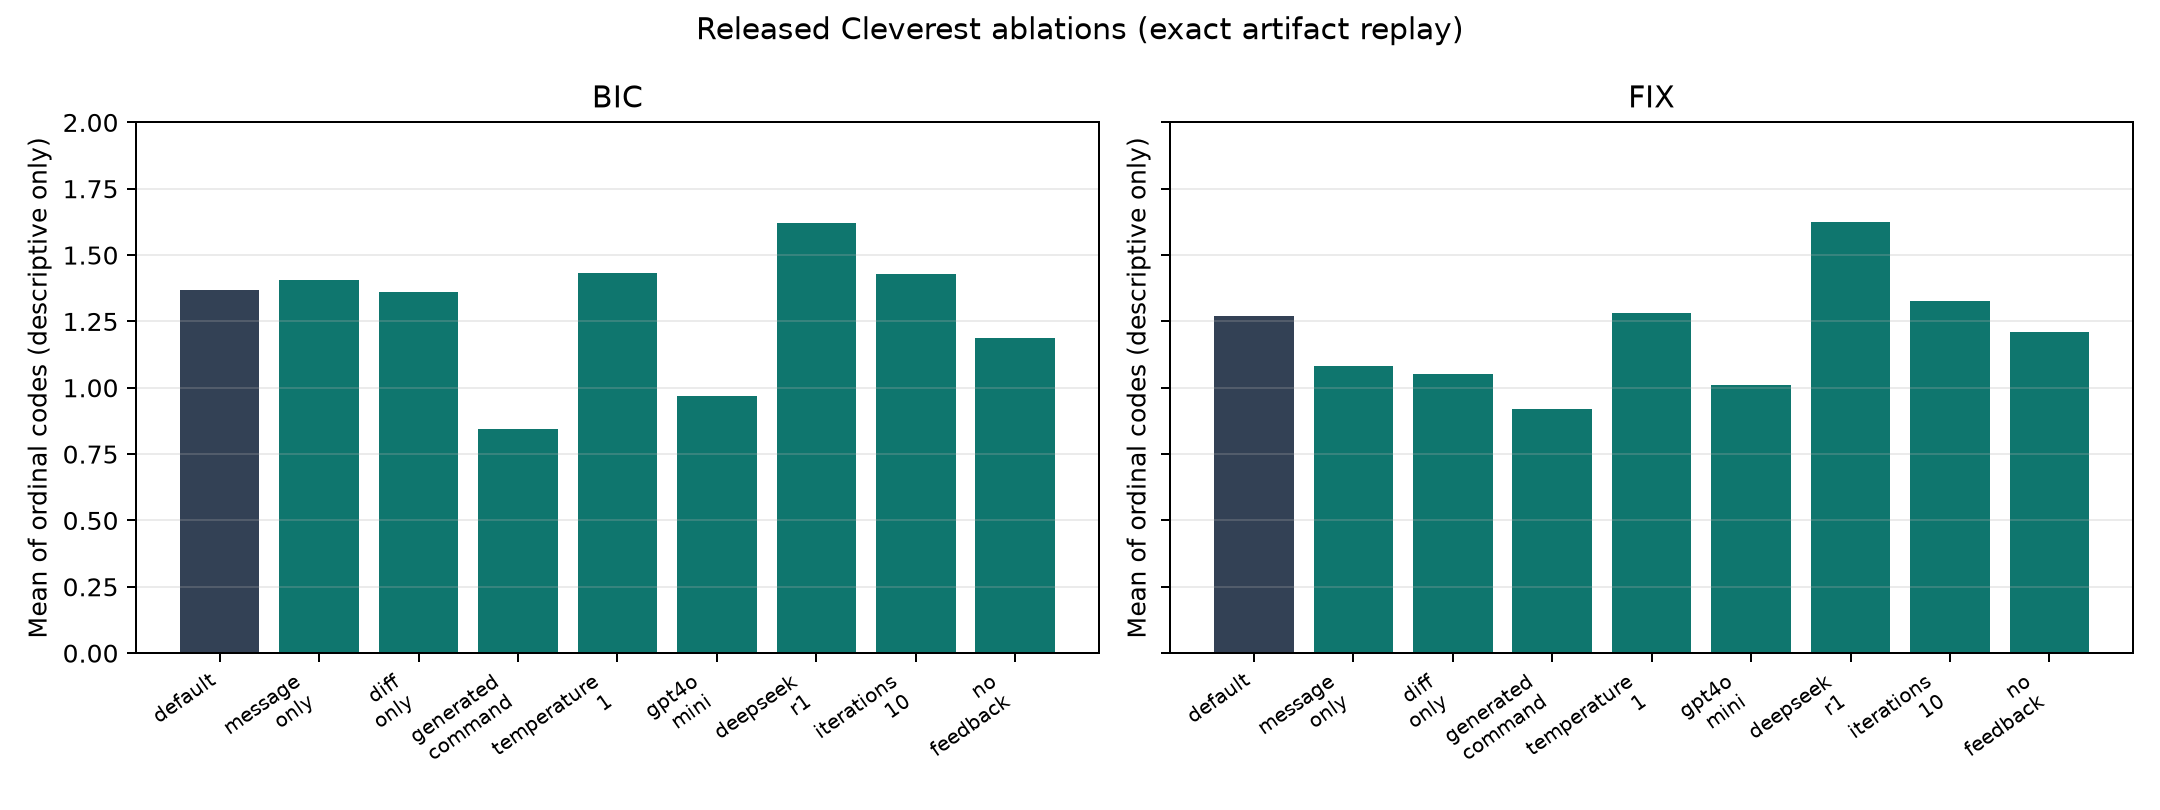
\includegraphics[width=\textwidth]{ablation_scores.png}
\caption{Exact descriptive replay of released ablation scores.  These bars are
not causal estimates and inherit the ordinal-scale assumption.}
\label{fig:ablations}
\end{figure}

\subsection{Data-dependent transformations}

The aggregator is not only a parser.  Across all rows, it converts 116 raw
\texttt{R} outcomes containing a \texttt{behave} status to score 2; converts
84 \texttt{X} outcomes with differing coarse crashes to score 2; assigns score
1 to four \texttt{X} rows after manual inspection; and changes one Poppler
message-only \texttt{D} to \texttt{N} because it could not be reproduced.
Source comments expose these decisions to artifact readers, which argues
against concealment.  Their frequency and adjudication protocol are absent
from the paper, and the final correction is explicitly post hoc.

%----------------------------------------------------------------------
\section{Validity and Comparison Audit}
\label{sec:validity}
%----------------------------------------------------------------------

\subsection{The headline equality pools opposite outcomes}

On the 50 commits where WAFLGo runs, Cleverest has 7 BIC and 11 BFC bug-any
successes; WAFLGo has 10 and 8.  Pooling gives the true arithmetic equality
$18=18$, but hides that Cleverest loses the paper's motivating bug-finding
scenario and wins reproduction.  ``In 24 hours'' is a campaign budget and
censoring convention, not the average time of successful WAFLGo discoveries.

The ClevFuzz union is 20/26 BIC and 18/24 BFC versus WAFLGo's 10/26 and 8/24.
Thus BFC is 2.25$\times$, but BIC is \emph{exactly} 2$\times$.  ``More than
twice in both scenarios'' is false.  The pooled 38 versus 18 does exceed two.

\subsection{Time accounting favors the narrative without reversing it}

The released notebook contains the assignments
\begin{lstlisting}[style=auditcode,numbers=none]
waflgo_result.loc[waflgo_result["init"] == "B", "success"] = 10
waflgo_result.loc[waflgo_result["init"] == "B", "time"] = 24 * 3600
\end{lstlisting}
Thus an initial corpus that already crashes is simultaneously a 10/10 success
and a 24-hour time-to-exposure.  These values contribute to reported means of
19:39:50 (BIC) and 21:48:32 (BFC).  Replacing five such entries per scenario
with zero reduces means by $5\cdot24/26\approx4.62$ hours and
$5\cdot24/24=5$ hours, to roughly 15.0 and 16.8 hours.  ClevFuzz's released
means are 5.7 and 6.2 hours.  The speed ordering therefore survives this
sensitivity analysis, but the magnitude falls.

\subsection{Significance is asserted but not tested}

The paper uses ``significantly'' for model power, message enhancement,
ClevFuzz, and directed versus undirected generation, while reporting no test,
confidence interval, effect size, or multiplicity procedure.  Our exploratory
checks illustrate why endpoint choice matters.  DeepSeek changes BIC bug-any
by four gains and one loss (exact McNemar $p=.375$) while changing mean ordinal
score by +0.253 (issue bootstrap 95\% interval +0.125 to +0.394; unadjusted
Wilcoxon $p=.0012$).  In BFC it has eight gains and one loss
($p=.039$) and a +0.356 mean-code shift.  These data support a model-dependent
association, not the causal statement that performance scales with model
\emph{size}; vendor, architecture, reasoning, serving, and training all differ,
and GPT-4o's parameter count is not public.

Temperature 1 changes the BFC mean by only +0.014 with an interval crossing
zero.  The paper nevertheless infers greater test diversity, a construct never
measured.  No-feedback lowers mean code but raises issue-level bug-any from
7 to 10 BIC and 13 to 14 BFC.  ``Feedback is crucial'' therefore depends on the
ordinal aggregate rather than the ultimate bug endpoint.

%----------------------------------------------------------------------
\section{Hindsight, Leakage, and CI Realism}
\label{sec:leakage}
%----------------------------------------------------------------------

\subsection{Target-specific commands leak future information}

The default model receives a per-issue command and options.  This is not always
a generic harness.  JQ issue \#3262 receives
\texttt{jq .[54E100]=7 @@}; the rare value central to the trigger is already in
the command.  Libxml2 rows receive combinations such as
\texttt{--recover --dropdtd --sax1 --nofixup-base-uris}.  For BFC reproduction,
a bug report may legitimately provide such a command.  For BIC bug finding,
the eventual report and PoC occur after the commit and cannot be available in
the proposed just-in-time CI use case.

The paper discloses the command and runs GENCMD, so this is not covert cheating.
It is nevertheless target and temporal leakage.  GENCMD covers 14 issues (28
commits) and sharply lowers score.  A clean notebook emits a stale warning
because its comment expects 220 rows while the data correctly contain
$14\cdot2\cdot10=280$.

\subsection{Memorization analysis does not rule out memorization}

The paper computes normalized Indel similarity~\cite{rapidfuzz_ratio} between
generated inputs and online PoCs.  Low character overlap cannot exclude a
semantically equivalent trigger, a memorized committed regression test, or
issue recall keyed by an issue number.  Removing a keyword and observing lower
performance distinguishes ``uses the keyword'' from ``ignores the keyword'';
it does not distinguish reasoning from keyword-cued memory.  At least JQ's
CVE-2025-49014 postdates GPT-4o's documented October 2023 knowledge cutoff, so
an assertion that every target predates the cutoff would also be incorrect.

\subsection{RQ3 mixes oracle information with selection effects}

Gemini-2.5-Flash receives the original commit and corresponding ground-truth
bug report; humans verify inclusion of key bug elements.  The enhanced Z3
\#7252 message states nested \texttt{re.loop} and bounds 0/1, nearly a prose
reproduction recipe.  Enhancement is applied to 29 not-already-perfect cases,
while reduction is applied to 22 already-reaching cases.  Floor, ceiling, and
regression-to-the-mean all favor the predicted directions.  There is no
irrelevant-word or blind-paraphrase control.

Relative to message-only on the selected 29 cases, the mean-code shift is +0.70
(bootstrap +0.39 to +1.04; Wilcoxon $p=.00027$), but bug-any has seven gains
and two losses (McNemar $p=.180$).  Calling the \emph{number of bugs}
significant is therefore unsupported by this natural issue-level test, even
though the ordinal shift is large.

\subsection{Known positives cannot establish no false positives}

All main subjects are retrospectively known buggy commits selected for
reproducibility.  This measures sensitivity conditional on selected positives,
not precision among ordinary commits, developer alert burden, or false-positive
rate.  System-level execution does not imply no false positives, and no method
is given for the assertion of no flakiness.  The 50-recent-commit experiment
closest to deployment is moved to supplementary material.

%----------------------------------------------------------------------
\section{Security and Evaluation-Integrity Findings}
\label{sec:security}
%----------------------------------------------------------------------

\subsection{LLM-generated command injection}

With GENCMD, the LLM controls a command string.  The guard only searches for
substrings \texttt{rm} and \texttt{sudo}; the result is later passed through
\texttt{script -c}.  Our exact parser/guard/constructor POC supplies:
\begin{lstlisting}[style=auditcode,numbers=none]
Command: `target @@; printf VERIFIED > /tmp/cleverest_cmd_injection_poc`
\end{lstlisting}
The constructed command is:
\begin{lstlisting}[style=auditcode,numbers=none]
timeout 30s /definitely/missing/build/target SAFE_INPUT;
printf VERIFIED > /tmp/cleverest_cmd_injection_poc
\end{lstlisting}
It creates the marker despite the intended executable failing.  Released
commands include \texttt{\$(python3 ...)}, confirming shell interpretation is
normal behavior.  A prompt-injected commit could influence the command; the
container has network access, runs as root by default, and receives an API key.
The default non-GENCMD Table~\ref{tab:default} does not use this path.

\subsection{Program output can forge the crash oracle}

\texttt{check\_output\_bug} searches combined pseudo-terminal output for text
such as \texttt{ERROR: AddressSanitizer:} and \texttt{Segmentation fault}.  It
does not establish stderr or sanitizer provenance.  Feeding its exact function
normal ``before'' output and target-printed ``after'' output produces:
\begin{lstlisting}[style=auditcode,numbers=none]
bug_before=''
bug_after=heap-buffer-overflow
classified_BIC_final=B
\end{lstlisting}
A generated program can condition printing on any version difference and turn
``output changed'' into ``bug.''  Searching 31,109 released inputs finds no
crash-marker string.  We therefore prove gaming potential and explicitly do
not claim exploitation.

\subsection{Fuzzer results lack intended-bug identity}

\texttt{checkfuzz.sh} counts a target-version crash if the other version does
not crash; if both crash, only equal coarse type strings are excluded.  There
is no stack/source match to a reference bug.  The result establishes a
differential crash, not necessarily \emph{the intended bug}.  CSVs contain
many correctly excluded same-both-side outcomes, but the released merged data
do not suffice to re-triage every success.  Actual ClevFuzz overcounting is
unresolved.

\subsection{Lower-severity boundaries}

Config files are sourced as shell code and must be treated as trusted.  The
Dockerfile downloads yq without a checksum, uses unpinned apt packages, names a
mutable base tag, and defaults to root.  Static inspection also finds copies
before \texttt{WORKDIR /clever} and an undefined \texttt{\$UNAME}; Docker was
unavailable, so runtime failure is not claimed.  The replication tar itself
contains no unsafe member.

%----------------------------------------------------------------------
\section{A Hardened Successor and the Twofold Target}
\label{sec:improvement}
%----------------------------------------------------------------------

We implement a benchmark-agnostic \texttt{cleverest\_plus} layer.  It requires
JSON with base64 input and an argv array; allowlists executable basenames;
rejects control operators, path escapes, substitutions, and multiple/missing
input placeholders; and invokes \texttt{subprocess.run} without a shell.  It
keeps stdout and stderr separate, parses sanitizer type and top frame, optionally
requires an expected reference signature, and treats any both-version crash as
ambiguous.  Cheap JSON, XML, PDF, and textual validation supports separate
valid/malformed candidate quotas.  Edge-set hashes select coverage-diverse
candidates.  Thirteen unit tests, Ruff, and BasedPyright pass.

The intended full pipeline is:
\begin{enumerate}[nosep]
  \item retrieve only commit-time-available issue/PR/history context;
  \item generate multiple structured candidates under a fixed token budget;
  \item validate and repair format while preserving a malformed-input quota;
  \item select edge-diverse candidates and feed uncovered changed lines back;
  \item synthesize only allowlisted argv from help text;
  \item minimize authentic crashers and run a short, budget-counted AFL++ phase;
  \item adjudicate against a reference stack signature.
\end{enumerate}

\begin{figure}[H]
\centering
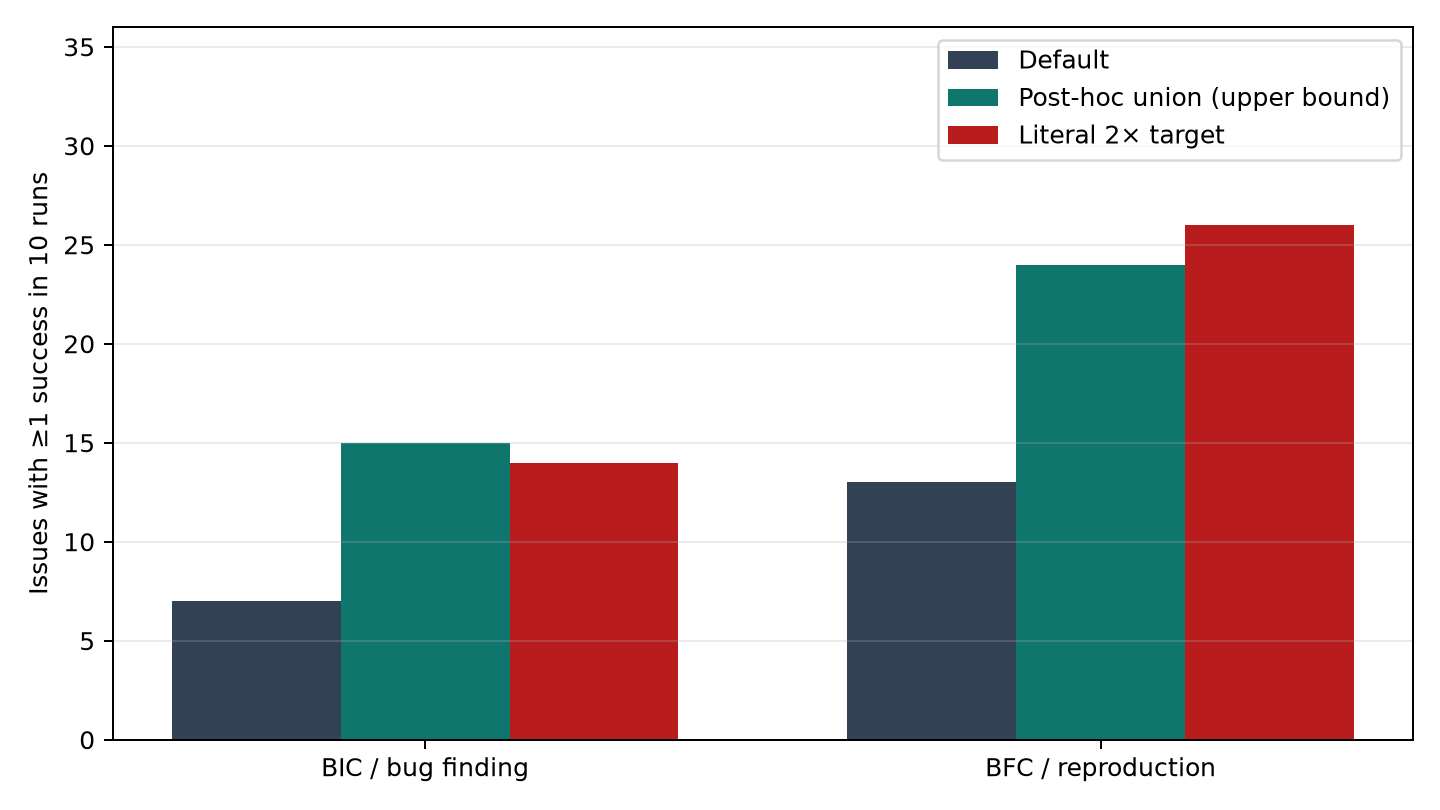
\includegraphics[width=.82\textwidth]{doubling_ceiling.png}
\caption{Default, retrospective union of released LLM configurations, and the
literal twofold target.  The union is an upper bound, not a prospective score.}
\label{fig:doubling}
\end{figure}

A post-hoc union of all released LLM configurations finds 15 BIC bugs versus 7,
exceeding the target 14.  It finds only 24 BFC bugs versus 13, below target 26.
DeepSeek plus temperature-1 has a retrospective BIC union of 14, but selecting
a pair after observing the benchmark and spending two configurations is not a
fair improvement result.  Full released ClevFuzz replay reaches 22/36 BIC and
20/36 BFC.  Neither available LLM nor hybrid data double BFC.

A defensible future experiment must preregister model snapshots, total tokens,
wall time (including fuzzing), primary endpoint, exclusions, transformations,
and statistics; use fresh post-cutoff or private commits; prohibit truth data
and future commands; run at least 30 independent campaigns where feasible; and
publish crash stacks.  Without credentials and Docker we cannot prospectively
run this protocol.  We decline to report a fabricated 2$\times$ score.

%----------------------------------------------------------------------
\section{Editorial Quality and ``AI Slop''}
%----------------------------------------------------------------------

The camera-ready says ``six open-source C programs'' although it evaluates
eight and includes C++ Z3.  The README says ``six'' while enumerating three plus
five.  It references out-of-table MicroPython \#13087 and JerryScript \#5155
instead of \#5153, says new programs have four to five bugs while MicroPython
has six, and labels a temperature-1 ablation \texttt{Temp0.x} in the rendered
Table 3.  The notebook expects 220 rather than 280 GENCMD rows.  Broken prose
includes ``introduce evaluate the utility'' and ``Issue \#550 of Libxml2 2.''
The Wittgenstein ``vibe testing'' passage is branding rather than evidence.

These are objective editorial defects and, in the last case, judgment about
relevance.  They are not an authorship classifier.  We cannot infer that an LLM
wrote the paper or that its data are fraudulent.

%----------------------------------------------------------------------
\section{Threats to This Audit}
%----------------------------------------------------------------------

We did not repeat proprietary generations, historical builds, or 24-hour
campaigns.  We did not contact authors, and some choices may have undocumented
benign explanations.  Our significance checks use issue means and issue-any
endpoints; other preregistered endpoints could be reasonable.  We report
unadjusted values only to diagnose unsupported language and do not present them
as confirmatory.  Stack identity would require raw crash artifacts absent from
the merged CSVs.  Security severity depends on deployment: command injection
inside a disposable no-secret/no-network container has lower impact than in an
ordinary CI worker.  Installing GNU grep on macOS was necessary to execute the
artifact's GNU-specific \texttt{-P} oracle parser.

%----------------------------------------------------------------------
\section{Conclusion}
%----------------------------------------------------------------------

Cleverest's released artifact earns substantial credit: complete transcripts
and inputs, exact configurations, checksummed archives, a dated default model,
and a raw-to-table pipeline we reproduce byte-for-byte.  We find no evidence of
fabrication or covert cheating.  The paper nevertheless confuses reproducible
numbers with strong inference.  Bug-specific future commands weaken the
zero-shot CI claim; scenario pooling and time conventions sharpen headlines;
RQ3 uses oracle-informed text and selected cases; ordinal averages and absent
statistics support causal/significance rhetoric; and vulnerable shell/oracle
boundaries allow evaluation gaming.

The productive response is not an allegation.  It is a stricter experiment and
a safer tool: time-respecting information, shell-free execution, authenticated
crash reports, stack identity, benign-commit precision, fresh targets,
preregistered budgets, and scenario-specific reporting.  Our hardened prototype
implements the core boundaries.  Available evidence doubles BIC only under a
post-hoc, higher-compute union and does not double BFC.  Scientific integrity
requires reporting that limit rather than optimizing the narrative.

\section*{Artifacts}
The HTML report, machine-readable analysis, POCs and outputs, reproduction log,
figures, and hardened prototype accompany this paper in
\texttt{./sorcar\_reported\_frauds/} and \texttt{./cleverest\_plus/}.

\bibliographystyle{plainnat}
\bibliography{cleverest_audit}

\end{document}
